%*************************************************
\section{Risk factors of malicious insiders}
\label{sec:riskMeasures}
%*************************************************
The risk posed by a potential MI has been identified as the top most devastating threat for the cloud ecosystem. Basically, a user or a software with authorized access to the cloud resources can be considered a MI. For preparation of an effective defense mechanism, first, with risk analysis the significance and scope of each threats posed by MIs should be characterized. Next, the mitigation solution proposed for each major risks. Among the different risk factors of a MI, the confidentiality and integrity violation of data are the most crucial security concerns. Evidently, the security mechanism provided by a CSP are vulnerable to the risk posed by a MI. Besides, using classic cryptographic schemes nullifies benefits of cloud computing and most of them leak critical information about underlying data. There are little initiatives designated to address the information leakage from encrypted data. The risk factors and the corresponding solutions as well as the advantages and disadvantages of the proposed solution are summarized in Figure\ref{fig:MIriskFactors}.

\begin{figure}[H]
\centering
\resizebox{0.9\textwidth}{!}{\begin{tikzpicture}[
block/.style={rectangle,draw,fill=gray!20,text width=9em,text centered,rounded corners,minimum height=4em,node distance=0.4cm,auto},
line/.style={draw,-latex',node distance= 2cm,auto}]

\node [block] (a) {Confidentiality violation};
\node [block, below=of a] (b) {Integrity violation};
\node [block, below=of b] (c) {Information leakage};

\node [block, right=of a] (sa) {Cryptosystems:\\AHOM, OPE, \\DET, RND };
\node [block, right=of b] (sb) { Query verification};
\node [block, right=of c] (sc) {1-Query tracking\\2-Selective insertion of disinformation};

\node [block, right=of sa] (aa) {1-Confidentiality\\2-Full control\\ over data};
\node [block, right=of sb] (ab) {Data authenticity};
\node [block, right=of sc] (ac) {1-Leakage limitation\\ 2-Indistinguishable info. and disinfo};

\node [block, right=of aa] (da) {1-Limited operations\\2-Computation cost};
\node [block, right=of ab] (db) {1-Computation cost\\2-Token overhead};
\node [block, right=of ac] (dc) {1-Data overhead\\2-Filter \& verification cost};

\path [line] (a) -- node {}(sa);
\path [line] (b) -- node {}(sb);
\path [line] (c) -- node {}(sc);


\path [line] (sa) -- node {}(aa);
\path [line] (sb) -- node {}(ab);
\path [line] (sc) -- node {}(ac);

\path [line] (aa) -- node {}(da);
\path [line] (ab) -- node {}(db);
\path [line] (ac) -- node {}(dc);

\node[label={\large Risk factor}]  at (-0.15,1) {};
\node[label={\large Mitigation}]  at (4.0,1) {};
\node[label={\large Advantage}]  at (8.5,1) {};
\node[label={\large Disadvantage}]  at (13.0,1) {};
\end{tikzpicture}
}
\caption{Risk factors of malicious insiders in the cloud DBaaS and the corresponding solutions with advantages and disadvantages}
\label{fig:MIriskFactors}
\end{figure}

The risk vector of MI is defined and modeled in the following subsection.

%*************************************************
\subsection{Risk model}
\label{MaliciousInsiderModelSubSec}
%*************************************************
Our approach to model a MI starts with identifying components and the associated risks as result of actions of a MI. Clearly, a MI in DBaaS infrastructure, has easier access and greater window of opportunity to does much severe harm than external attacker. A MI can bypass all internal protection mechanism and poses serious risks to perform \textit{confidentiality}, \textit{integrity} and \textit{inference} violation. The list of possible actions are denoted as $A=\{C, I,\Psi \}$ respectively. We assume that there are $n$ collections are stored in the data warehouse of DBaaS rephrased as: $W_{DBaaS}= \{D_1,\dots,D_n\}$.\\


\noindent A MI has read/write access in the data warehouse and activity log files denoted with $L$. Let $R$ present the key resources in the DBaaS $R=\{W_{DBaaS}, L\}$. A MI interested in sensitive information about an entity $\mathbb{T}$ as a target. Information about $\mathbb{T}$ is stored in the collection $D_i$ in form of document-store or set of $\langle key, value \rangle$ pair(s). The MI has one initial document stored in the one collection $D_i$, and his goal is to obtain sensitive attributes of $\mathbb{T}$. We analyze the associated risk factors of cloud DBaaS as a result of actions of a MI.\\


%*************************************************
\subsubsection*{Confidentiality violation risk}
\label{subsec:ConfidentialityViolation}
%*************************************************
A MI misuses the existing privileges to gain further access to sensitive information without any trace of intrusion. Internal attacks are very hard to detect because the users are authenticated on the domain.\\
\textbf{Mitigation:} Cryptographic schemes should be considered by the data owner to encrypt data before outsourcing it to the cloud. Meanwhile, processing over encrypted data without decryption is essential requirement that put restriction to cryptographic schemes selection.\\

\noindent A MI can extract an encrypted sensitive attribute $\hat{A}=\langle E_k(key), E_k(value) \rangle$ about $\mathbb{T}$ stored in collection $D_i$ by iteratively calling the correlation function to the rest of collections $\Psi (D_i, D_j)$. One single element can be classified in different level of importance in variety of organizations. The MI in DBaaS can exploit this  difference in the aggregated data pool to violate confidentiality of sensitive attributes. It can be shown that two collections $D_i$ and $D_j$ that initially do not share any documents, but later on it turns out to be they both have common documents that are describing the same entity $\mathbb{T}$. Therefore, the MI maintains a list of the explored collections, and we have a \emph{binomial distribution} with parameters $n \in \mathbb{N}$ as a number of collections and $p \in [0,1]$ as success probability of each collection. The problem is sampling with replacement and the probability of finding $k$ sensitive documents in $n$ collections of the cloud warehouse $W_{DBaaS}$. The reason for sampling with replacement is, If $\Psi(D_r, D_s)==false$, but due to discovery of a new correlation $\Psi(D_s, D_t)==true$ the new extracted attribute(s) can change $\Psi(D_r, D_s)$ to true. The function defining discrete probability distribution of $k$ documents from exploring $n$ collections is:   

\begin{equation}
\label{binomialDistribution}
f(k;n,p) = {{n} \choose {k}}p^{k}(1-p)^{n-k}
\end{equation}
The mean value and the variance of $f(k;n,p)$ are
\begin{equation}
median = n \times p  \qquad \sigma_{f} = n \times p (1-p).
\end{equation}

The probability of extraction one sensitive attribute from the $n$ collections is:
\begin{equation}
\label{oneSuccess}
f(1;n,p) = n\times p\times(1-p)^{n-1}
\end{equation}

The probability distribution of successful extraction of zero document related to the $\mathbb{T}$ from  entire $W_{DBaaS}$ is

\begin{equation}
\label{zeroSuccess}
f(0;n,p) = (1-p)^{n}.
\end{equation}
 
%*************************************************
\subsubsection*{Integrity violation (active attack) risk}
\label{subsec:IntegrityViolation}
%*************************************************
An integrity violation can happen in a cloud data store by unauthorized modification of data.\\
\textbf{Mitigation}: The \emph{integrity verification} mechanism ensures data is only modified by an authorized valid user, and identifies integrity violation done by an  MI. We introduced \emph{query integrity verification} tamper-resistant algorithm which is built on Message authentication codes (MAC). By appending a new attribute to each document denoted as \emph{eTag}, containing a value which is keyed hash value of whole document. Detail of this method is discussed in subsection \ref{QueryintegrityVerificationSubSec}.\\

Sensitive documents in the cloud DBaaS are in risk of unauthorized modification by a MI. Maintaining data integrity in the stored collections is a crucial necessity in the outsourced datasets. Detection of unauthorized modification can be done by Message Authentication Code (MAC) over sensitive documents. Similar to digital signature, MAC appends an authentication \textit{eTag} to any document. The building block of MAC is a keyed-hash function to generation/verification of eTag. A data owner generates $\langle eTag, E_k(d_i)\rangle$ and appends as a new attribute to all given documents, later on the verification process grantees the authenticity and integrity of documents as presented in Equation \ref{eTag}.   
\begin{equation}
\label{eTag}
\begin{aligned}
&Verification: \\
&eTag^{'}= MAC_k(document); \begin{cases}
&if (eTag==eTag^{'}) \implies ~ Document~is~valid.\\
&else~ Document~ is~ invalid. 
\end{cases}
\end{aligned}
\end{equation}



%*************************************************
\subsubsection*{Information leakage risk}
\label{subsec:ConfidentialityViolation}
%*************************************************
Encrypted databases are prone to information leakage, for instance deterministic and OPE cryptographic schemes always leak frequency and the order of plaintext data respectively. Subsequently, with a simple frequency analysis or sorting attack, MIs are able to obtain sensitive information. Later on, with an inference attack they combine leaked data with information in the other databases in the same cloud DBaaS or a public domain to hack the database.
 
\textbf{Mitigation}: We propose a method of Selective Disinformation Document Padding (SPDP) to hinder information extraction, while avoiding overhead of disinformation document padding. SPDP uses diagnostic metrics such as precision, recall and statistical analytics to periodically probe the dataset for the existence of the possible explicit and/or implicit correlations between data elements. Thereafter, the detected leakage is compared to the maximum acceptable level of leakage. If the result exceeds the maximum level (determined by the data owner), SPDP generates a certain number of fake documents to be inserted into the dataset in order to decrease the amount of leaked information. The number of generated disinformation documents depends on the significance of the leakage metrics.\\

The flexibility of NoSQL databases in terms of having different number of attributes corresponding to each document, helps us to create light-weight documents in order to mitigate data overhead in the DBaaS server. All the original and disinformation documents are encrypted and semantically indistinguishable from the MI’s point of view. The ciphertext dataset is processed by a standard cloud DBaaS, in a similar way to the plaintext data. In addition, the indexes in database are used to improve query processing time by shrinking the search space. Correspondingly, by indexing the encrypted data elements, a remarkable improvement is achievable in query processing time.

The dynamic nature of a dataset as a persistent storage necessitate to have basic operations to create, read, update and delete (known as CRUD). The augmented dataset (with disinformation documents), naturally are subjected to CRUD operations.  The create and read operations act on the augmented dataset in a similar way to a normal dataset, while the update/delete operations on the original documents should be projected on the corresponding disinformation documents. For the performance purpose, the update/delete operations on the related disinformation documents, can be processed on demand or postponed to the next period of the data analysis.
Furthermore, the garbage collector service, run by the proxy, can be developed to delete any unrelated disinformation from the dataset. The design and development of such a service is beyond the scope of the current work. 

The probability for the one attribute to be extracted from $n$ collections is given by Equation \ref{oneSuccess}. For leakage minimization purpose, at the any leakage points $\mathcal{V}$ disinformation documents generated and inserted to the collection. The leakage point are detectable by using the two methods that are introduced in this work. In particular, insertion of $\mathcal{V}$ disinformation documents creates $\mathcal{V}$ branches from each one of documents to the other correlated documents. Ultimately, the result is a full tree-like structure with $\mathcal{V}+1$ branch factor which requires exponentially computation from MI to extract number of attributes. The number of branches in proportional to height $h$ is:    

\begin{equation}
\label{numberOfNodes}
N = 1+\mathcal{V}+ \mathcal{V}^2+ \dots + \mathcal{V}^h= \frac{\mathcal{V}^{h+1}-1}{\mathcal{V}-1}.
\end{equation}

Thus, the new probability distribution function is
\begin{equation}
\label{attibutesFromDilutedDB}
f(k;n,p) = \prod_{i=0}^{\mathcal{V}} {{N} \choose {k}}p^{\frac{k}{i}}(1-p)^{N-k}.
\end{equation}

%*************************************************
\subsection{Query integrity verification}
\label{QueryintegrityVerificationSubSec}
%*************************************************
DBaaS could be subject of passive or active attack by a MI. In passive attack an attacker attempts to uses all tools and credentials to gain information about a specific target without changing the data. Particularly, passive attacks are designed to violate confidentiality of the targeted entity. However, in an active attack, the MI exploits cloud DBaaS to conduct unauthorized data modification on the target. In other word, the goal of an active attack is integrity violation.\\

To address the query integrity verification, we propose a method that effectively identifies and filters out the invalid documents from query response at the proxy side. First, the data owner adds a new attribute to the original documents, denoted as \emph{eTag}. Next, a single token is required to identify valid documents, i.e. a 32-byte secret keyword. In order to achieve data integrity and eliminate the risk of unauthorized data modification, we considered a document digest which is computable by a cryptographic hash function. In the next step, the data owner needs to encrypt the concatenation of token and digest with RND cryptosystem for each of the documents to store the output as a value for eTag. Now, it is time to create $\mathcal{V}$ number of disinformation documents with minimum precision and recall value to be inserted into the dataset. For instance, for a collection containing $10^6$ documents and $\mathcal{V}=10$, we need to insert $10$ fake documents per each original document in the collection. According to semantic security principle, the original and fake documents should be indistinguishable. Thus, the same steps for creation of eTag are needed to be conducted for the fake documents with a new token for identification purpose.

In particular, each valid document is an equivalent class for $\mathcal{V}$ documents that have diverse value for semi-identifier attributes to prevent identity disclosure. Because of this feature this method is denoted as $\mathcal{V}$- anonymity. Finally, the attributes of real and fake documents are encrypted according to the security plan and forwarded to the DBaaS in the cloud. Figure \ref{fig:QueryIntegrityVerification} illustrates the process of eTag calculation for the documents.

%Figure
\begin{figure}[H]
\centering
\resizebox{0.7\textwidth}{!}{\tikzset{
table nodes/.style={
rectangle,
draw=black,
align=center,
minimum height=6mm,
text depth=0.5ex,
text height=2ex,
inner xsep=0pt,
outer sep=0pt
},      
table/.style={
matrix of nodes,
row sep=-\pgflinewidth,
column sep=-\pgflinewidth,
nodes={
    table nodes
},
execute at empty cell={\node[draw=none]{};}
}
}
\tikzstyle{doc}=[%
draw,
thick,
align=left,
color=black,
shape=document,
minimum width=8mm,
minimum height=5mm,
]
\begin{tikzpicture}[scale=0.8,align=left]
\node (Info)[doc,fill=green!20, fill opacity=0.5,text opacity=1] {
\begin{tikzpicture}
\node[label={\textbf{Info doc}}] (A) at (-10,0) {};
\matrix (B) [table,text width=15mm,below =-4mm of A, ampersand replacement=\&]
{
$Key_1$     \& $Value_1$\\
...         \& ...\\
$Key_n$     \& $Value_n$\\
};
\end{tikzpicture}
};
\node (DisInfo)[doc,below=2mm  of Info,fill=red!20, fill opacity=0.4,text opacity=1] {
\begin{tikzpicture}
\node[label={\textbf{Disinfo doc}}, color=black] (A) at (0,0) {};
\matrix (B) [table,text width=15mm,below =-5mm of A,  ampersand replacement=\&]
{
$Key_1$     \& $Value_1$\\
...         \& ...\\
$Key_n$     \& $Value_n$\\
};
%\node [rectangle,text width=0.1cm,minimum height=0em,right= of B] (C) {};
\end{tikzpicture}
};
\node[box1, fill=gray!20, fill opacity=0.3,text opacity=1, every text node part/.style={align=left}] (Enc) at (7,-1) {{\normalsize \\$Digest = Hash\{Document\}$\\ $eTag:\bm{E_k\{Token\Vert Digest\}}$};

\node[box1, fill=gray!20, fill opacity=0.4,text opacity=1, every text node part/.style={align=left}] (eTag) at (14.5,-1) {{\underline{Encryption}}\\ \\{ $E_k(Key_1):E_k(Value_1)$} \\.. \\$E_k(Key_n):E_k(Value_n)$};
\node (EncDoc)[doc,below=0.5  of eTag,fill=white, fill opacity=0.1,text opacity=1] {
\begin{tikzpicture}
\node[label={\textbf{Encrypted doc}}, color=black] (ED)  {};
\matrix (B) [table,text width=22mm,below =-5mm of ED, ampersand replacement=\&]
{
$\color{red} \bm{eTag}$ \&$\color{red}\bm{value}$\\
$E_k(Key_1)$     \& $E_k(Value_1)$\\
...         \& ...\\
$E_k(Key_n)$     \&$E_k(Value_n)$\\
};
\end{tikzpicture}
};

\node (EncDoc2)[doc,fill=white,fill opacity=1.0,text opacity=1]  at (13.5,-7.0) {
\begin{tikzpicture}
\node[label={\textbf{Encrypted doc}}, color=black] (ED)  {};
\matrix (B) [table,text width=22mm,below =-5mm of ED, ampersand replacement=\&]
{
$\color{red} \bm{eTag}$ \&$\color{red}\bm{value}$\\
$E_k(Key_1)$     \&$E_k(Value_1)$\\
...         \& ...\\
$E_k(Key_n)$\&$E_k(Value_n)$\\
};
\end{tikzpicture}
};
\draw[->, >=latex, black!70, line width=4pt,rotate=-90]   (DisInfo) to node[black]{} (Enc) ;
\draw[->, >=latex, black!70, line width=4pt,rotate=-90]   (Info) to node[black]{} (Enc) ;
\draw[->, >=latex, black!70, line width=4pt,rotate=-90]   (Enc) to node[black]{} (eTag) ;
\draw[->, >=latex, black!70, line width=4pt,rotate=-90]   (eTag) to node[black]{} (EncDoc) ;

\end{tikzpicture}}
\caption{The high level diagram of \textit{query integrity verification } technique.}
\label{fig:QueryIntegrityVerification}
\end{figure}

The proxy decrypts eTag value with the decryption key and verifies the tag of original documents from the query response and filters out the disinformation documents. The MAC are used to protect against any unauthorized modifications of documents. With the mechanism of digital signature that implemented in eTag, the proxy verifies the authenticity of whole document with recalculation of document digest and verification with the digest. The digital signature of the documents adds a small overhead to the documents, however it guarantees the document never gets modified by cloud insiders. Intuitively, eTag is not involved in a query processing and this attribute will be used for the internal structure for providing integrity of data store.\\

In order to minimize the information leakage, we propose to encrypt attributes which are low level granularity with RND cryptosystems. Equation \ref{eq:NonDeterminsticEncryption} outlines RND (non-deterministic) encryption function constructed from a deterministic one. First we associate a unique fixed length random number $r$, with each document. With application of eTag, the risk of active attack and unauthorized modification by third party is detectable in the verification phase in the proxy.


\begin{equation}
\label{eq:NonDeterminsticEncryption}
\begin{aligned}
& E_k (x) = E^{\prime}_k (x \left\lvert \right\rvert r) \\ 
\end{aligned}
\end{equation}
\textbf{Where:}\\
\begin{minipage}[b]{0.5\textwidth}
\raggedright
{\bf k} is the encryption key\par
{$\boldsymbol{E^{\prime}}$} is a DET encryption.
\end{minipage}%
\begin{minipage}[b]{0.5\textwidth}
\raggedright
{\bf r} is a random number.
\end{minipage}
\newline

The crypto-hash functions are building blocks of the introduced query integrity verification algorithm, and therefore, having an efficient hash function leads to low latency integrity verification. We examined the performance of four popular hash functions according to the variety of document size. The result is displayed in Figure \ref{fig:hashPerformance}. Considering the performance and security metrics, we select \emph{SHA1} over other hash functions including MD5, RIPEMD and SHA256 to be used in eTag algorithm. As it can be observed from Figure \ref{fig:hashPerformance}, the reason of selection of SHA1 is its high performance (speed) at different input documents sizes.

%Figure
\begin{figure}[H]
\centering
\resizebox{0.6\textwidth}{!}{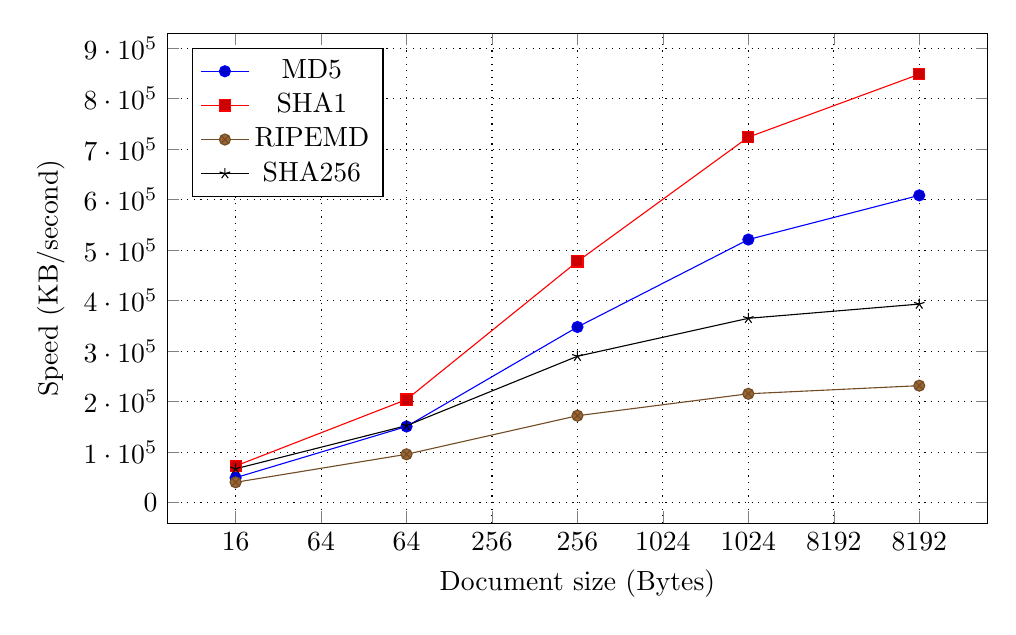
\begin{tikzpicture}
\begin{axis}[legend style={at={(0,0)},anchor=west,at={(axis description cs:1.05,0.45)}},    title={},
ytick={0,100000,200000,300000,400000,500000,600000,700000,800000,900000},
symbolic x coords={16,64,256,1024,8192},
%ytick=data,
xlabel={Document size (Bytes)},
ylabel={Speed (KB/second)},
scaled y ticks=false, 
compat=newest, %Better
legend pos=north west,
%axis background/.style={fill,bottom color=gray!50,top color=white},
grid=major,
height=7.8cm,width=12cm,
grid style={dotted,black}
]
\addplot+ coordinates {
	(16,49292.32)      %16
	(64,150689.13)     %64
	(256,347740.76)    %256
	(1024,520933.03)   %1024
	(8192,608428.03)   %8192
};
\addlegendentry{MD5}
\addplot+ coordinates {
	(16,72490.62)      %16
	(64,204046.66)     %64
	(256,477543.25)    %256
	(1024,723760.47)   %1024
	(8192,848322.56)   %8192
};
\addlegendentry{SHA1}
\addplot+ coordinates {
	(16,40183.96)      %16
	(64,95633.13)      %64
	(256,172034.90)    %256
	(1024,215498.41)   %1024 
	(8192,231541.42)   %8192
};
\addlegendentry{RIPEMD}
\addplot+ coordinates {
	(16,66921.74)      %16
	(64,152366.29)     %64
	(256,289791.49)    %256
	(1024,364940.63)   %1024 
	(8192,393106.77)   %8192
};
\addlegendentry{SHA256}
\end{axis}
\end{tikzpicture}}
\caption{Performance of four popular cryptographic hash functions in respect to document size.}
\label{fig:hashPerformance}
\end{figure}

\noindent The information leakage due to attribute correlation is investigated in the next section.